% \phantomsubsection
\subsubsection{Benefits of 3D Plotting:} \label{sec:benefits_of_3d_plot}
    \vspace*{-0.4cm}
    \begin{focus}
        % \item Super useful when combining visualizations of multiple objects, for example combining HMI with AIA Image or adding a LASCO Map.
        % \item For Example, PFSSPy, a dependent of SunPy, has a feature of overplotting field lines over an AIA Map, such a feature would be benefited a lot if there is 3D plot support in SunPy. (\autoref{fig:pfsspy}).
        % \item Good for intuitive understanding and visualization.
        % \item Looks super cool.
        \item Super helpful when combining visualizations of multiple objects, for example combining HMI with AIA Image or adding a LASCO Map.
        \item Moreover, PFSSPy, a dependent of SunPy, which calculates the Potential-Field Source-surface modelfor computing the coronal magnetic field features, has an exciting attribute, which can overlap field over the image. One of the best use-cases of 3D plotting in SunPy (\autoref{fig:pfsspy}).
        \item Suitable for intuitive understanding and visualization.
        \item Looks super cool.
    \end{focus}
    \begin{figure}[H]
        \centering
        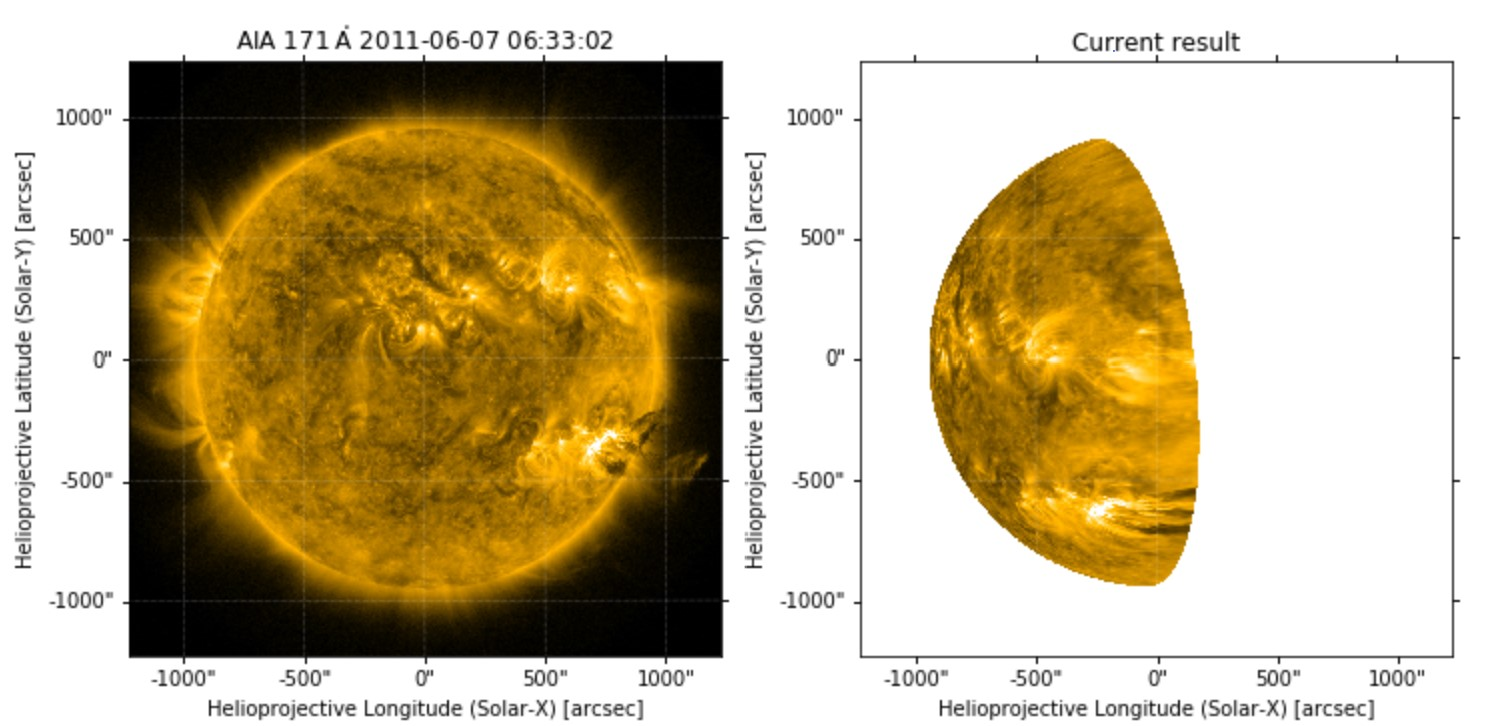
\includegraphics[scale=0.5]{figs/fig_3d_1.jpg}
        \caption{Example for show-casing usefulness of 3D plots, Issue \# 3997}
        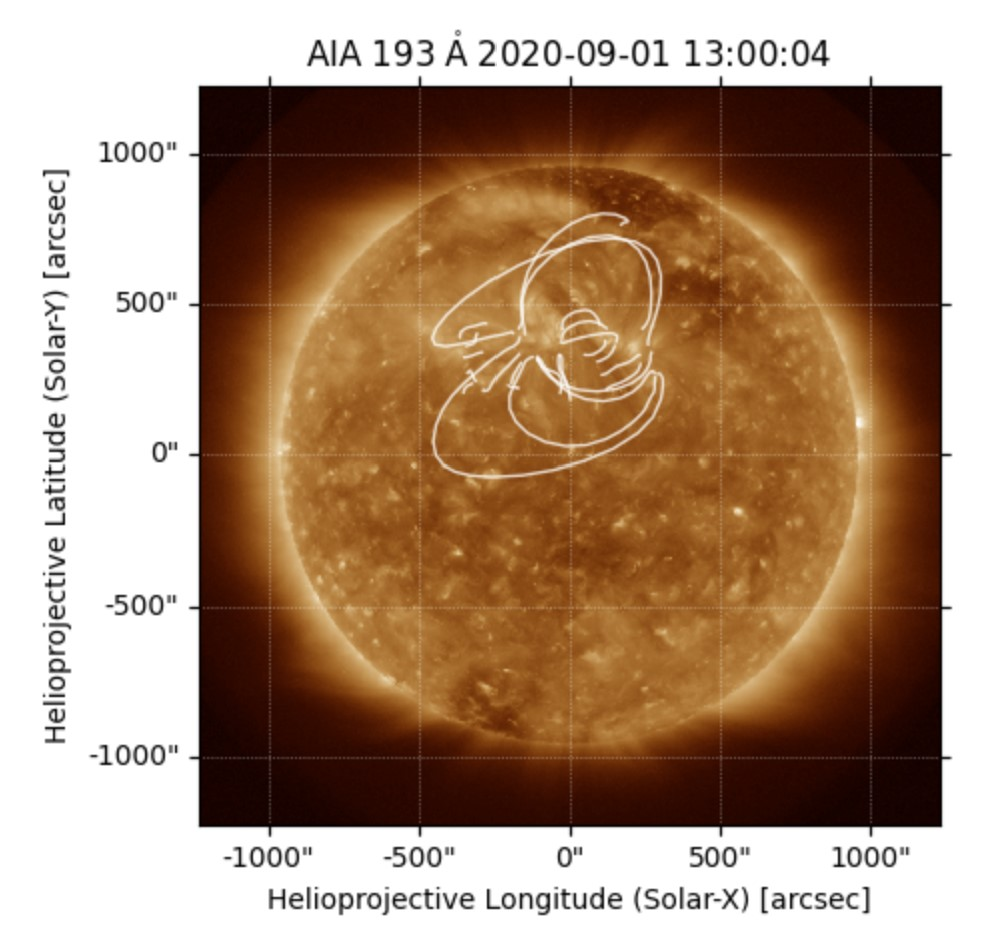
\includegraphics[scale=0.5]{figs/fig_3d_pfss_2.jpg}
        \caption{Overplotting field lines over an AIA Map with PFSSPy}
        \label{fig:pfsspy}
    \end{figure}
